\section{Study Data Collection and Topic Modeling} \label{sec:methodology}
In this Section, we discuss our data collection process to find  LCSD related posts (Section \ref{data_collection}). We then discuss the details of the topic modeling (Section \ref{topic_modeling}).
 
\subsection{Data Collection} \label{data_collection}
We collect  LCSD related SO posts in three steps: \begin{inparaenum}[(1)]
\item Download SO data dump,
\item Identify  LCSD related tag list, and
\item Extract  LCSD related posts from the data dump based on our selected tag list.
\end{inparaenum} We describe the steps below.

\nd\textbf{Step 1: Download SO data dump.} We downloaded SO data dump~\cite{SOdump} of June 2020. We used the contents of Post.xml file, which contained information about each post like the post's unique ID, type (Question or Answer), title, body, associated tags, creation date, view-count, etc. Our data dump included posts from July 2008 to May 2020 and contained around 58,544,636 posts. Out of them, 33.4\% are questions, 66.6\% are answers, and 17.4\% questions had accepted answers.

\nd\textbf{Step 2: Identify low-code tags.}
We need to identify the tags that are related to LCSD in order to extract low-code related posts from SO discussions.
To find relevant tags, we followed a similar procedure used in prior work~\cite{abdellatif2020challenges, ahmed2018concurrency, wan2019discussed, linares2013exploratory}. At Step 1, we identify the initial low-code related tags and call them $T_{init}$. At Step 2, we finalize our low-code tag list following related work~\cite{bagherzadeh2019going, yang2016security}. Our final tag list $T_{final}$ contains 19 tags from the top nine LCDPs. We discuss each step in details below.

(1) Identifying Initial low-code tags.
The SO posts do not have tags like ``low-code'' or ``lowcode''. Instead, we find that  low-code developers use a  LCSD platform name as a tag, e.g., ``appmaker'' for Google Appmaker~\cite{googleappmaker}. Hence, to find relevant tags, first we compile a list of top  LCSD platforms by analysing a list of platforms that are considered as the market leaders in Gartner~\cite{vincent2019magic}, Forrester~\cite{rymer2019forrester}, related research work~\cite{sahay2020supporting}, and other online resources like PC magazine~\cite{pcmag}. We find nine  LCSD platforms are consistently mentioned in the above resources: Zoho Creator~\cite{zohocreator}, Google App Maker~\cite{googleappmaker}, Salesforce Lightning~\cite{salesforce}, Quickbase~\cite{quickbase}, Outsystems~\cite{quickbase}, Mendix~\cite{mendix}, Vinyl~\cite{vinyl}, Appian~\cite{appian}, and Microsoft Powerapps~\cite{powerapps}. %In addition, several other  LCSD platforms are mentioned sporadically in some sources like Kissflow~\cite{kissflow} and ProntoForms~\cite{prontoforms}, but whose discussions are non-existent in our SO data dump. 
We thus focus on the discussions of the above nine LCSD platforms in SO. We find one tag per  LCSD platform as the name of the platform (e.g., ``salesforce-lightning''). 
However, upon close inspection of the tags in SO, we found that developers used more than one tag for some of the nine  LCSD platforms. For example, ``Microsoft Powerapps'' has multiple tags (e.g., ``powerapps'', ``powerapps-formula'', ``powerapps-canvas''). At the end of both quantitative analysis and manual validation by four authors, we found a total of 16 tags for the nine  LCSD platforms. We refer to these 16 tags as $T_{init}$. 

% our choice of initial 16 and the final 19 tags was based on both quantitative analysis and manual validation by four co-authors. 


(2) Finalizing low-code related tags.
Intuitively, there might be more variations to tags of nine  LCSD platforms other than those in $T_{init}$. We use heuristics from previous related works~\cite{bagherzadeh2019going, yang2016security} to find other relevant tags. First, we denote our entire SO dump data as $Q_{all}$. Second, we extract all the questions $Q$ that contain any tag from $T_{init}$. Third, we create a candidate tag list $T_{candidate}$ using all the tags found in questions $Q$. Fourth, we select significantly relevant tags from  $T_{candidate}$ for our  LCSD discussions. Following related works~\cite{bagherzadeh2019going, yang2016security}, we compute significance and relevance for each tag $t$ in $T_{candidate}$ with respect to $Q$ (our extracted questions that has $T_{init}$ tag) and $Q_{all}$ (i.e., our data dump) as follows,
{ \[
( Significance) \ \ S_{tag} \ =\ \ \frac{\#\ of\ ques.\ with\ the\ tag\ t\ in\ Q}{\ \ \#\ of\ ques.\ with\ the\ tag\ t\ in\ Q_{all}}
\]

\[
% ( Relevance) \ \ \mv \ =\ \ \frac{\#\ of\ questions \ with\ the\ tag\ t\ in\ Q}{\ \ \#\ of\ the\ questions\ in\ P}
( Relevance) \ \ R_{tag} \ =\ \ \frac{\#\ of\ questions\ with\ tag\ t\ in\ Q}{\ \ \#\ of\ questions\ in\ Q}
\]} A tag t is significantly relevant to  LCSD if the $S_{tag}$ and  $R_{tag}$ are higher than a threshold value. We experimented with a wide range of values of $S_{tag}$ and  $R_{tag}$. We found relevant tag set for  LCSD for $S_{tag}$ = 0.2 and $R_{tag}$ = 0.005 . These values are consistent with related work~\cite{bagherzadeh2019going,ahmed2018concurrency}. The final tag list $T_{final}$ contains 19 significantly relevant tags. 
%that also contains the 16 tags from $T_{init}$.


\nd\textbf{Step 3: Extracting low-code related posts.}
An SO question can have at most five tags, and we consider a question as low-code related question if at least one of its tag is in our chosen tag list $T_{final}$. Based on our $T_{final}$ tag set, we found a total of 7,302 posts from our data dump. There were 51.3\% Questions (i.e., 3,747) and 48.7\% Answers (i.e., 3,555) and among them 16.9\% Questions (i.e., 1,236) had accepted answers. SO has a score-based system (upvote and downvote) to ensure the questions are in proper language with necessary information (code samples and error messages), not repeated or off-topic. Here is an example for a question with score ``-4'' where a practitioner is making an API related query in Powerapps(\dq{61147923})\footnote{$Q_i$ and $A_i$ denote a question Q or answer A in SO with an ID $i$} platform. However, it is not clear what the practitioner is asking as the question is poorly written and without any clear example. In order to ensure good quality discussions, we excluded questions that had a negative score which resulted in 6,982 posts containing 51.5\% Questions (i.e., 3,597 ) and 48.5\% Answers (i.e., 3,385). Following previous research~\cite{bagherzadeh2019going, rosen2016mobile, barua2014developers}, we excluded unaccepted answers and only considered accepted answers for our dataset. Hence, our final dataset $B$ contained  4,785 posts containing 3,597 non-negative scored questions and 1,188 accepted answers. 
%and their metadata to conduct this study. 



\subsection{Topic Modeling} \label{topic_modeling}
We produce  LCSD topics from our extracted posts in three steps: \begin{inparaenum}[(1)]
\item Preprocess the posts, 
\item Find optimal number of topics, and
\item Generate topics.
\end{inparaenum} We discuss the steps below.

\nd\textbf{Step 1. Preprocess the posts.} For each post text, we remove noise following related works~\cite{abdellatif2020challenges,bagherzadeh2019going,barua2014developers}. First, we remove the code snippets from the body, which is inside \textless code\textgreater \textless /code\textgreater\ tag, HTML tags such as (\textless p\textgreater \textless /p\textgreater, \textless a\textgreater \textless /a\textgreater, \textless li\textgreater \textless /li\textgreater\ etc), and URLs. Then we remove the stop words such as ``the'', ``is'', ``are'', punctuation marks, numbers, non-alphabetical characters using the stop word list from MALLET~\cite{mccallum2002mallet}, NLTK~\cite{loper2002nltk}, and our custom low-code specific (i.e.,  LCSD platform names) stop word list. After this, we use porter stemmer~\cite{ramasubramanian2013effective} to get the stemmed representations of the words e.g., ``wait'', ``waits'', ``waiting'', and ``waited'' - all of which are stemmed to base form ``wait''.

\nd\textbf{Step 2. Finding the optimal number of topics.}  After the prepossessing, we use Latent Dirichlet Allocation~\cite{blei2003latent} and the MALLET tool~\cite{mccallum2002mallet} to find out the  LCSD related topics in SO discussions. We follow similar studies in Software engineering research using topic modeling~\cite{arun2010finding, asuncion2010software, yang2016security, bagherzadeh2019going,abdellatif2020challenges}. Our goal is to find the optimal number of topics $K$ for our dataset $B$ so that the \textit{coherence} score, i.e., encapsulation of underlying topics, is high. We use Gensim package~\cite{rehurek2010software} to determine the coherence score following previous works~\cite{uddin2017automatic, roder2015exploring}. We experiment with different values of $K$ that range from \{5, 6, 7, .., 29, 30\} and for each value, we run  MALLET LDA on our dataset for 1000 iterations~\cite{bagherzadeh2019going}. Then we observe how the coherence score is changing with respect to $K$. We pick the topic model with the highest coherence score. Choosing the right value of $K$ is important because, for smaller values of $K$, multiple real-world concepts merge, and for a large value of $K$, a topic breaks down. For example, in our result, the highest coherence score 0.50  for $K$ = 7 and $K$ = 13. We choose $K$ = 13 as it captures our underlying topics better. For $K$ = 7, we find that it merges the topics ``Dynamic Event Handling'', ``Dynamic Content Display'', and ``Dynamic Form Controller''. MALLET also uses two hyper-parameters, $\alpha$ and $\beta$, to distribute words and posts across the topics. Following the previous works~\cite{bagherzadeh2019going, ahmed2018concurrency, bajaj2014mining, rosen2016mobile}, we use the standard values $50/K$ and 0.01 for hyper-parameters $\alpha$ and $\beta$ in our experiment.  

\nd\textbf{Step 3. Generating topics.} Topic modeling is a method of extracting a set of topics by analysing a collection of documents without any predefined taxonomy. Each document has a probability distribution of topics, and every topic has a probability distribution of a set of related words~\cite{barua2014developers}. We produced 13 topics using the above LDA configuration on our dataset $B$. Each topic model offers a list of top $N$ words and a list of $M$ posts associated with the topic. In our settings, a topic consists of 30 most frequently co-related words, which represents a concept. Each post had a correlation score between 0 to 1, and following the previous work~\cite{wan2019discussed}, we assign a document with a topic that it correlates most. 







% https://stackoverflow.com/questions/61147923/how-to-parameterize-api-url-in-powerapps
% \paragraph{Step 4: LDA Topic Modeling.}
% 
% \textit{Preprocess the posts} 
% Before we run the topic modeling on our extracted questions, we need to preprocess them. For the topic modeling we used posts title, body and accepted answers. Then we followed the following steps to remove noise from our documents following related works \cite{abdellatif2020challenges} \cite{bagherzadeh2019going} \cite{barua2014developers}. First we remove the code snippets from the body which is inside \textless code\textgreater \textless /code\textgreater\ tag, HTML tags (\textless p\textgreater \textless /p\textgreater, \textless a\textgreater \textless /a\textgreater, \textless li\textgreater \textless /li\textgreater\ etc), URLs. Then we remove the stop words such as "the", "is", "are", punctuation marks, numbers, non-alphabetical characters using the MALLET'S stop word list\cite{} and ?. After this we use stemmer to get the stemmed representations of the words e.g., "wait", "waits", "waiting", "waited" all were stemmed to base form "wait".
% % prunning remove words appeared more than ? percent or less than ? percent
% % to preprocess i.e. stop words removal, lematization, prunning etc. We followed the best guidelines on how to apply topic modeling in Software Engineering research\cite{chen2016survey}
% 
% 
% \textit{Topic modeling settings}
% % Defination of topic modeling
% Topic modeling is a method of extracting a set of topics by analysing a collection of documents \cite{wiki1} without any predefined taxonomy. In this method each document has a probability distribution of topics and every topic has a probability distribution of set of related words \cite{barua2014developers}. For example, we have a topic called ? which consists of high frequency words such as ?,? ,? ? etc. 
% 
% % Topic modeling tools, configuration, settings, and some results
% After the prepossessing, we used Latent Dirichlet Allocation  \cite{blei2003latent} and the MALLET tool \cite{mccallum2002mallet} to find out the low-code development related topics that are discussed on SO. We followed similar studies in Software engineering research using topic modeling \cite{asuncion2010software} \cite{yang2016security} \cite{bagherzadeh2019going} \cite{abdellatif2020challenges}. 
% 
%  Choosing the right value of K is important because for smaller value of K multiple different real world concepts will be merged and for large value of K a topic will be broken down to some subtopic. For example when we used K = ? ? and ? topic were merged into one. And when we used K = ?, ? topic was divided into ? and ? subtopic. In our experiments we experiments, we tried different values of K ranges from {5, 6, .? ? ?. , 30}. and I = {1, 43,243 ,? ? }. We used coherence metric value to find for which value of K the topics have more understand-ability \cite{roder2015exploring}. We found that when K value ranges ? to ? the coherence score is very high and almost same. Based of manual observation of top ? topics we found that for K=? the model generates good topics for our low-code dataset. For MALLET configuration we used the standard values 50/K and 0.01 for hyper-parameters $\alpha$ and $\beta$  which provided good results for us following previous work \cite{bagherzadeh2019going} \cite{ahmed2018concurrency} \cite{bajaj2014mining} \cite{rosen2016mobile}. In our settings, a topic consists of ? most frequently co-related used words which represents a concept. After ? iteration the Mallet returns a K topics and each topic consists of ? words.
% 
% 
% \textit{Labeling topics}
% LDA usually captures topic by analysing SO discussions without proper understanding of domain-specific concepts. 
% Mallet does not provide a meaningful title for the topic, it only returns a set of co-related words. 
% % We need to name to K topics returned by the Mallet a meaningful name.
% We need to categorize the K LDA topics on technical discussions returned by the MALLET to match higher level concepts. For example, a topic with group of words were ...??... 
% 
% From previous works \cite{}\cite{} \cite{} we used open card sort \cite{fincher2005making} to label the $K$ topics. In this way we inspected ? words in each topic and read top ? posts associated with that topic to come up with a topic name. From the $K$ topics we merged topic ? with topic ? because after analysing the posts it seemed like they were basically mentioning same things. The topics were discussed by all the authors in. In order to categorize topics into higher level category we grouped similar topics. For example topic ? and topic ? were grouped into ? higher level topic. Table \ref{} shows the summary of topic names, high level category name, favorite count, number of posts in each topic etc.
% 
% 
% % LDA also provided to find similarity of between topics
% 
% 
% 
% 
% \paragraph{Step 5: Manually label questions to understand practitioner's challenges}
% Manually labelling the questions to understand the challenges the low-code application practitioners are facing was the most time consuming part of this study. We conducted X round of meetings over X months to plan, discuss and resolve conflicts. At the end we need less regular meetings because we were already in sync. In total we reviewed X number of SO questions and among them around X\% of questions required conflict resolution meeting. 
% 
% We analysed and labeled the extracted posts by four authors in a open coding procedure \cite{seaman1999qualitative}. The questions extracted at step 3, were divided among three authors who labeled a question by providing a description of the challenge. The number of labels were growing very diverse as there are not much clarification and guidelines to categorize the low-code development challenges. So we decided to label each question on a fixed list of tags. Initially we started with 84 tags summarized from authors' label of the challenge. Some of this tags very closely related for example ? ? ?.  We routinely held meetings and updated this list either by introducing new tags or merging some of the existing tags together. For example we merged ? and ? to ? because they were closely related. Again after labeling a few questions we introduced ? tag because we saw there were lots of questions regarding that. This way we were able to maintain a consistent naming without suffering a significant bias \cite{humbatova2020taxonomy}.
% 
% The goal of this manual review of SO discussion was to fully understand what sort of challenges the practitioners are facing, so we studied the questions along with answers and comments to fully understand the real issue and provide a label to it. We spent around 3 hours for the questions labeling and resolving conflicts. There were some questions which were vague to understand which we labeled ?. We rigorously followed procedures in labelling the questions, specially for the tricky situations like 1. Questions was not related low-code application rather some general programming language related. 2. authors did not understand how to tag/label this question.
% 
% A final meeting was held and we reviewed the tag list and number of questions in each tag. We merged some of tags that had relatively very low number of questions.
% 
% % Some of the questions are tagged wrongly because the citizen developers do not have enough domain knowledge to tag appropriately. Applying right tag is important to get proper support from community experts \cite{bangash2019developers}.
% 
% % open card sorting \cite{spencer2009card}
% 
% 
% 
% \paragraph{Step 6: Taxonomy of challenges Construction \& Validation.}
% 
% % \begin{figure*}[htb]
% % \centering
% % 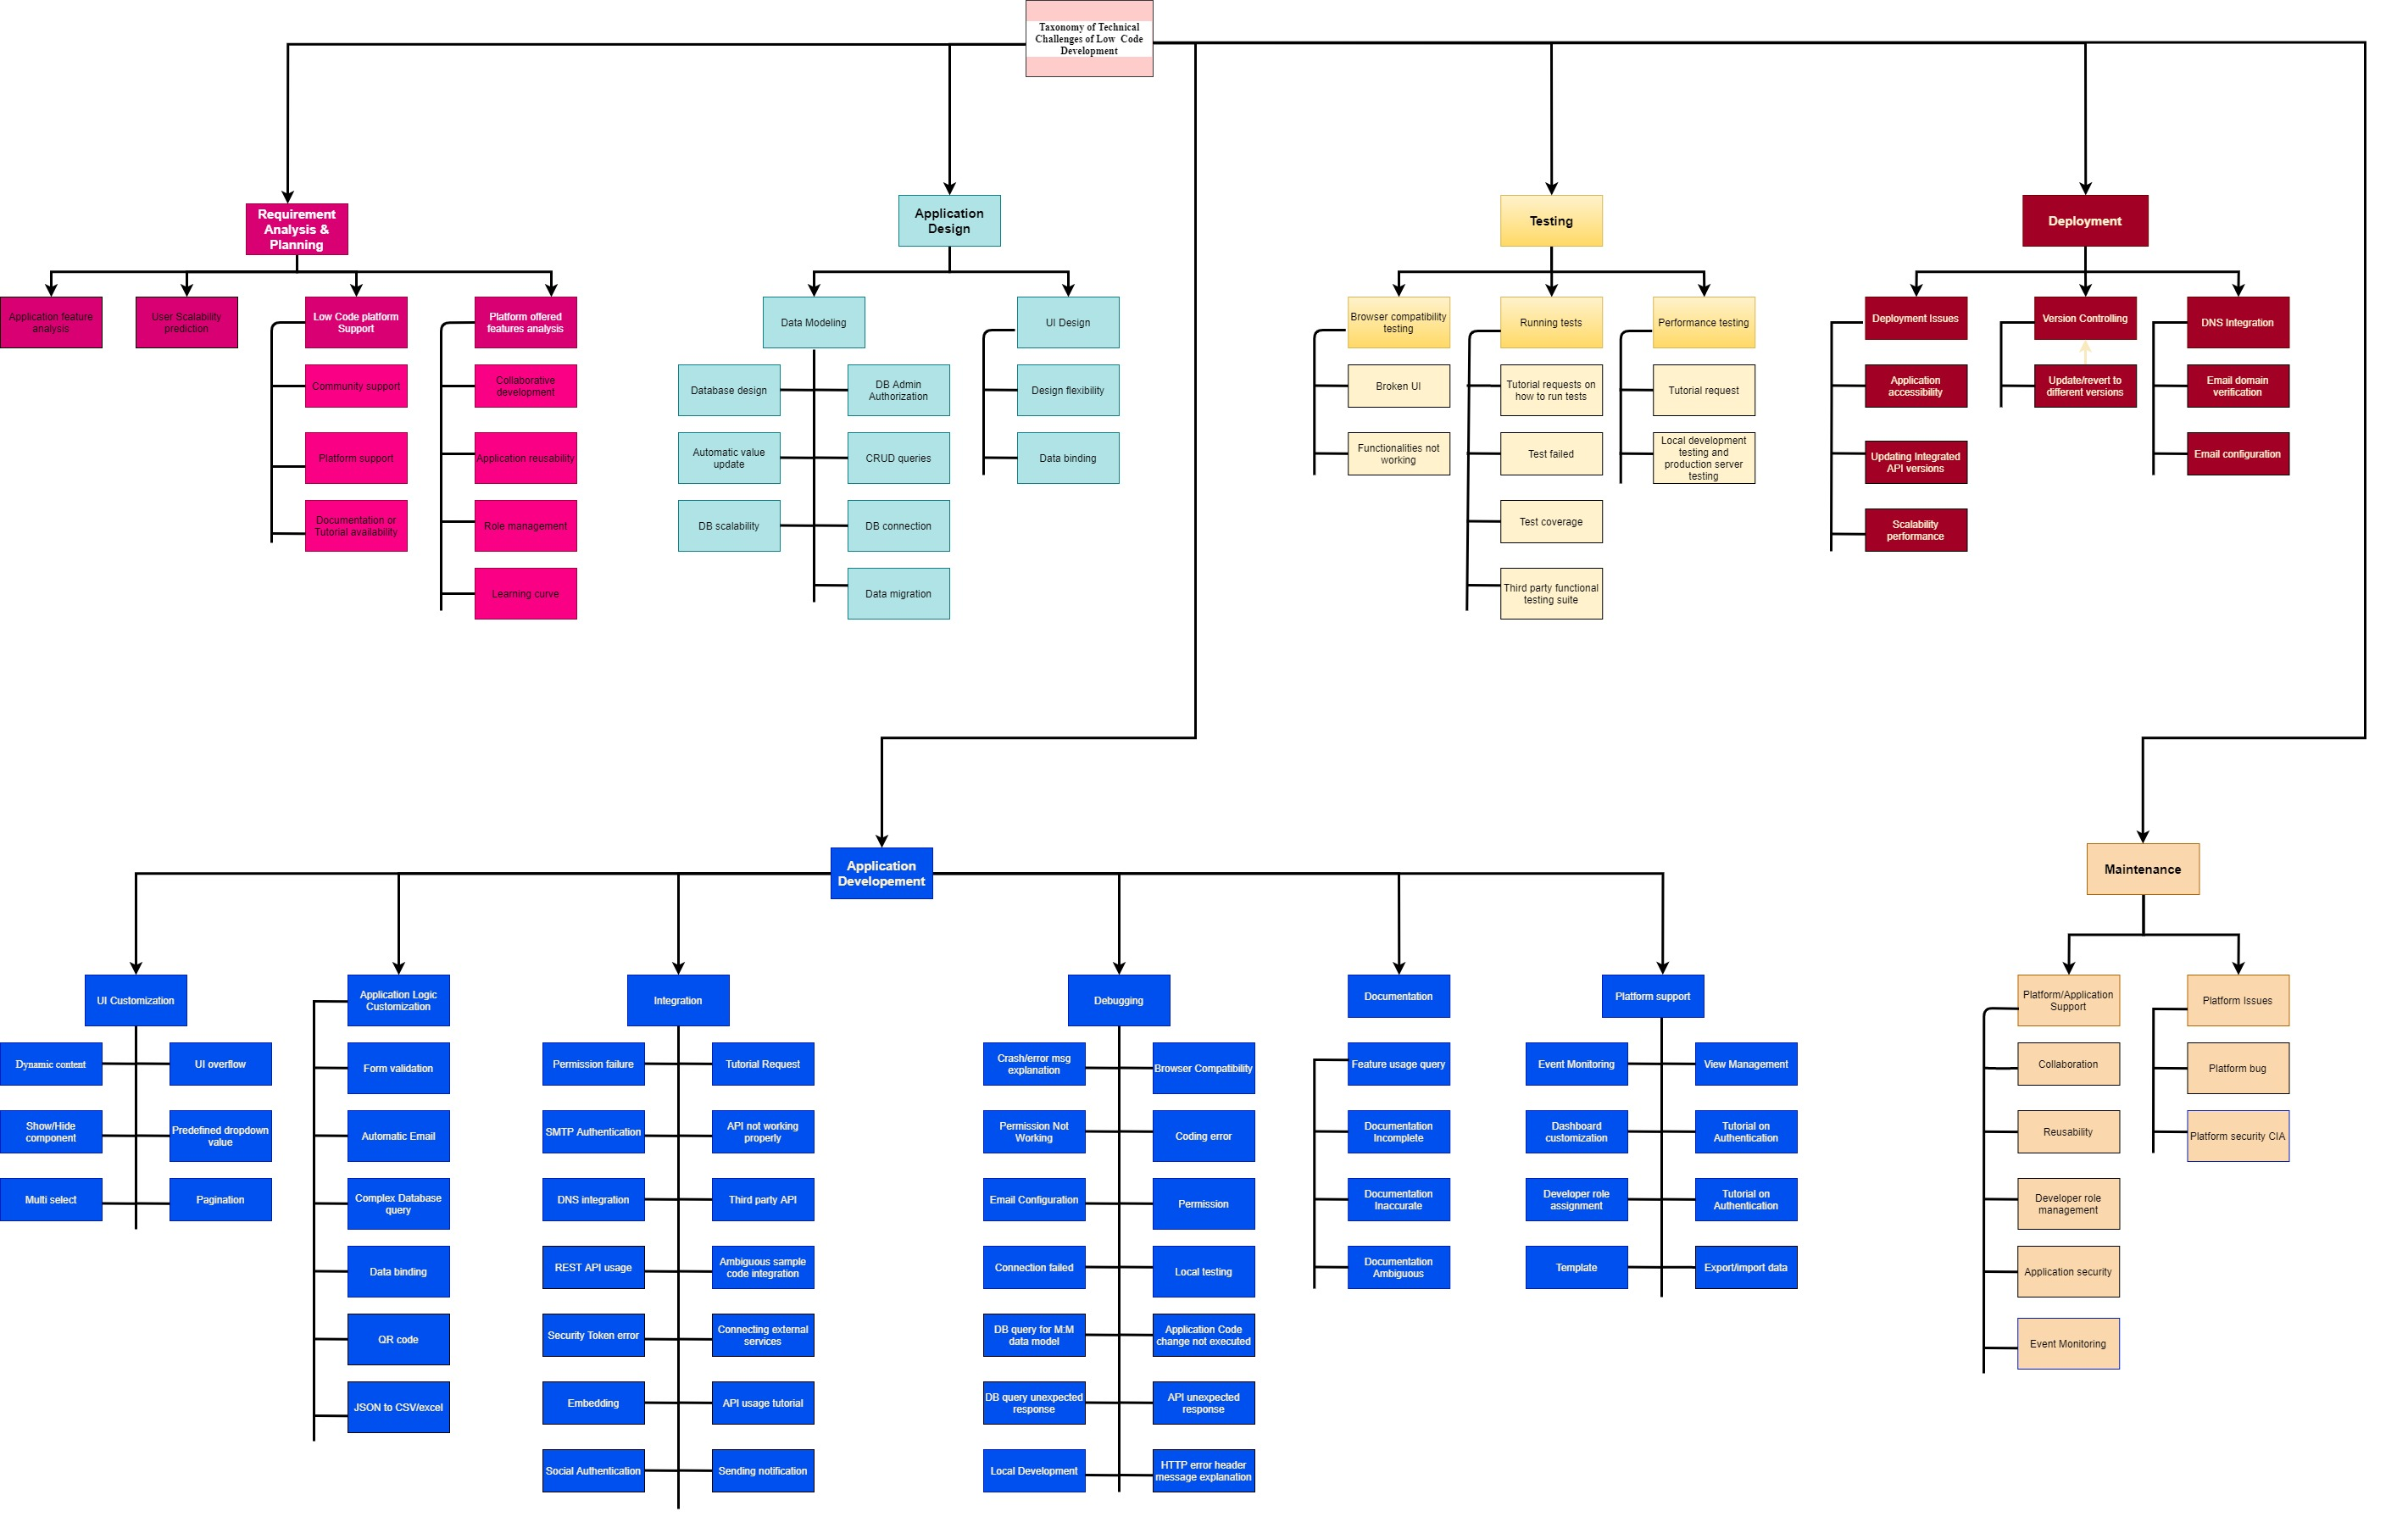
\includegraphics[scale=0.17]{res/LowCodeChallenges.jpg}
% % % 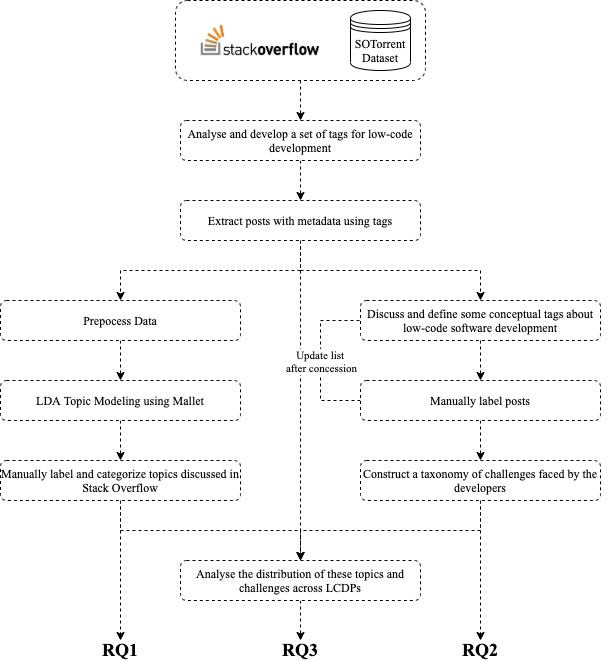
\includegraphics[width=0.35 * linewidth]{res/methology_overview.jpg}
% % \caption{Taxonomy of challenges that low-code practitioners face during different life cycle of application development}
% % \label{fig:taxonomoy_low_code_challenges}
% % \end{figure*}
% 
% we built the taxonomy is a bottom up approach\cite{humbatova2020taxonomy}. First we created a group for similar tags and then we created a high-level classification of the parent category. Each classification was validated by all the authors in a group meeting. At the end all of the authors reviews the categories, subcategories and sub sub categories and made some final changes.
% 
% We organized our taxonomy based the challenges practitioners face during different phases of application development . Our taxonomy consists of ? higher level category resembling the ? stages of agile software development life cycle. Each SDLC stage contains some sub-category of challenges that low-code practitioners have discussed on SO. There are total ? sub category of challenges such as ? ? ?. Each of this sub-category contains some low level low-code technology related challenges i.e. tags. In total there are ? low level tags. Figure \ref{sec:taxonomy}.
% 
% The final taxonomy is reviewed and agreed with all the authors. We had some reservations with the initial taxonomy that we resolved by discussing it with each other.
% 
% 
% \paragraph{Step 7: Analyze discussions and challenges across LCDPs.}
% 
% 
% 
% % From our extracted data we found that in total ? LCDPs are discussed in SO. 
% 



